\documentclass{article}
\usepackage[top=0.5in,bottom=1in,left=1.25in,right=1.25in]{geometry}
\usepackage{hyperref,setspace,graphicx,amsmath,amssymb,booktabs,array,float}
\usepackage{tikz,pgfplots}
\usetikzlibrary{arrows.meta,positioning,shapes.geometric}
\usepgfplotslibrary{groupplots}
\pgfplotsset{compat=1.18}
\hypersetup{colorlinks=true,linkcolor=blue,citecolor=blue,urlcolor=blue}
\setlength{\emergencystretch}{2em}
\title{\textbf{Observability-Aware Trust-Based Grayhole Detection for Underwater Acoustic Networks}}
\author{}
\date{}
\begin{document}
\setstretch{1.5}
\maketitle
\section*{Team Members}
\noindent 241CS110, Appaji Nagaraja Dheeraj, \texttt{appajidheeraj.241cs110@nitk.edu.in}\\
241CS111, Aryan Bokolia, \texttt{aryanbokolia.241cs111@nitk.edu.in}\\
241CS117, Karthikeya Gupta, \texttt{karthikeyagupta.241cs117@nitk.edu.in}

\section*{Abstract}
\noindent
Underwater acoustic networks rely on relay nodes to carry sensor data to a surface sink, and a grayhole relay can secretly drop part of that traffic. The classic defence is a watchdog that listens for each forward and accuses a relay whose missed forwards exceed a fixed threshold. Underwater, however, forwards are also missed because of half-duplex deafness, collisions at the relay and long, lossy acoustic links, and these losses grow with traffic. A fixed watchdog therefore catches grayholes only by also accusing honest nodes, and routing around those honest nodes costs delivery and throughput. This work implements, in UnetStack, a network-layer detector that judges only windows the monitor could have observed, compares the forwards heard with the number an honest relay should show on each link given its distance and the normal loss of its area, combines monitors as an area-weighted trust value, and flags relays with a dynamic threshold and two-round confirmation. The sink receives the evidence as reports over the acoustic channel, gives the administrator a ranked suspect list and routes traffic around confirmed grayholes. In 12-hour simulations on ten test networks with one, two and three grayholes, the detector caught 95\% of the grayholes while accusing 0.3 honest nodes per run, against 7.2 for the fixed watchdog, and gave the highest delivery ratio and throughput of the compared methods.

\section{Introduction}\label{sec:intro}
\subsection{Background and challenges}
Underwater sensors often need intermediate relays to deliver measurements to a sink. Acoustic communication introduces propagation delay and half-duplex operation: a node cannot receive normally while it transmits. UnetStack provides the protocol agents and modem notifications needed to study these interactions in simulation~\cite{unet}. This project concerns network-layer forwarding; physical-layer events supply monitoring evidence.

A watchdog listens for a neighbour to forward a packet. Failure to overhear that forward has several possible causes. The neighbour may have deliberately dropped the packet, may never have received it, or may have forwarded it while the monitor failed to decode the transmission. The original watchdog literature already identifies collision-related limitations~\cite{marti}. The problem is therefore not solved by assigning a trust score to every silence.

Several challenges affect evaluation as well as design. Filtering more windows can reduce false accusations simply by discarding evidence. Different monitors can observe the same packet, so their counters are correlated. A learned normal-loss estimate can itself be contaminated by attackers. Finally, a detector that performs well with complete offline evidence may perform differently when reports must cross a lossy network.

\subsection{Problem statement and objectives}
We investigate whether locally observable conflict checks and expected-loss correction can improve grayhole detection relative to explicitly defined baseline adaptations. The method must use monitor observations rather than attacker labels, and its performance must be assessed together with false accusations and reporting cost.
\begin{enumerate}
\item Implement and explain a watchdog that distinguishes retained forwarding windows from locally unobservable windows.
\item Compare the proposed detector, a fixed watchdog, a CAD-style adaptation and component variants on the same recorded traffic, with thresholds tuned on separate networks that are never used for testing.
\item Measure delivery, delay and transmission cost when detection, reporting and route response occur in time order.
\end{enumerate}
The study does not aim to establish immunity to false reports, field performance, or superiority over complete implementations of every published protocol.

\subsection{Organization}
Section~\ref{sec:related} positions the work and identifies the implemented comparators. Section~\ref{sec:method} gives the model and algorithm. Section~\ref{sec:experiments} defines the experiments and metrics. Section~\ref{sec:results} reports detection and network outcomes. Section~\ref{sec:limits} discusses validity and limitations, followed by the conclusion in Section~\ref{sec:conclusion}.

\section{Literature Review}\label{sec:related}
\subsection{Watchdog monitoring}
Marti et al. introduced watchdog monitoring together with pathrater-based routing~\cite{marti}. The monitor retains packet information and checks for a matching retransmission. The paper discusses ambiguous collisions, receiver collisions and partial dropping among its limitations. Its advantage is that forwarding can be checked through overhearing; its limitation is that silence does not uniquely identify the cause of loss. Our fixed-rate watchdog is an inspired comparator, not a reproduction of the full watchdog/pathrater system.

\subsection{Channel-aware detection}
Shila et al. estimate normal losses caused by channel impairment and medium-access collisions, then compare measured loss with the normal-loss estimate~\cite{cad}. Their published CAD method includes upstream and downstream monitoring and adaptive detection thresholds. This establishes that channel correction and adaptive thresholds are existing ideas. Our CAD-style comparator retains a downstream channel/collision correction using monitor busy time. It omits the published upstream protocol, probe/acknowledgement exchange and signed reports. Its performance therefore cannot establish a win over the complete published CAD algorithm.

\subsection{Selective forwarding in UnetStack}
Chandavarkar and Suresh demonstrate selective forwarding and a detection mechanism in UnetStack3~\cite{brc}. The supplied implementation description uses destination-side timeouts and forwarding counters. It motivates studying the attack in an underwater networking stack, but is not the sender-overhearing comparator used in our experiments. We extend the project question toward local observability, expected loss and a ranked suspect list rather than claiming to reproduce that paper.

\subsection{Underwater trust-aware routing}
Han et al. combine trust evaluation and fuzzy logic with layered underwater routing~\cite{han}. Their model addresses forwarding selection using trust and neighbourhood information. This provides relevant context for using trust in an underwater network, but does not itself validate our observation filter or formulas. We do not implement their routing protocol as an experimental baseline.

\subsection{Comparison and scope of the contribution}
\begin{table}[H]\centering\small\setstretch{1}
\begin{tabular}{p{2.7cm}p{4.5cm}p{5.1cm}}\toprule
Approach & Useful idea & Boundary of this comparison\\\midrule
Watchdog~\cite{marti} & Overhear forwarding & Our comparator uses a fixed miss-rate threshold, not full pathrater.\\
CAD~\cite{cad} & Estimate channel and collision loss & Our downstream adaptation is not full CAD.\\
UnetStack3 study~\cite{brc} & Demonstrate selective forwarding & Destination-timeout method is not reproduced here.\\
Trust-aware routing~\cite{han} & Use trust in forwarding selection & Background work, not a measured comparator.\\
Proposed method & Filter local conflicts; pool expected-forward evidence & Known positions/channel curve; honest reports; simple static simulation.\\\bottomrule
\end{tabular}
\caption{Positioning of the project. The table does not establish that no earlier method uses related ideas.}
\end{table}
The specific contribution evaluated here is the combination of stated per-window exclusions, distance-informed expected forwards and a dynamic decision rule in this UnetStack setting. Component comparisons test whether the exclusions add value to the same estimator. A comprehensive novelty assessment remains separate from demonstrating this project-level improvement.

\section{Proposed Approach}\label{sec:method}
\subsection{Baseline watchdog and our modifications}
The baseline is the classic watchdog used to demonstrate selective-forwarding detection in UnetStack3. Each sender acts as a monitor of its next hop and follows two rules:

\textit{Rule 1: after sending a packet to the next hop, listen for its forward; a forward not heard in time is a miss.}

\textit{Rule 2: if the fraction of misses exceeds a fixed threshold (30\%), accuse the next hop.}

Underwater, a forward can be missed although the relay is honest: the monitor itself was transmitting (half-duplex), the packet collided at the relay, or the long acoustic link lost it. These losses grow with traffic, so the fixed threshold accuses honest relays, and routing around them forces detours and lowers delivery. Taking into account what an acoustic node can actually observe, the following modifications were made:
\begin{itemize}
\item \textbf{Observability:} a window counts only if the monitor could have heard the forward; hidden windows are ignored instead of being counted as misses.
\item \textbf{Trust from each link's expected loss:} expected forwards are computed per link from its distance and the normal loss of its distance area (near, medium, far), and trust is heard divided by expected forwards, combined over all monitors as an area-weighted average.
\item \textbf{Evaluation with a dynamic threshold and confirmation:} a relay is flagged only when its shortfall is significant for the current network, and becomes a suspect only after two flagged rounds in a row; confirmed grayholes leave the baseline so further grayholes stand out.
\end{itemize}
Figure~\ref{fig:beforeafter} contrasts the two decision paths.
\begin{figure}[H]\centering\setstretch{1}
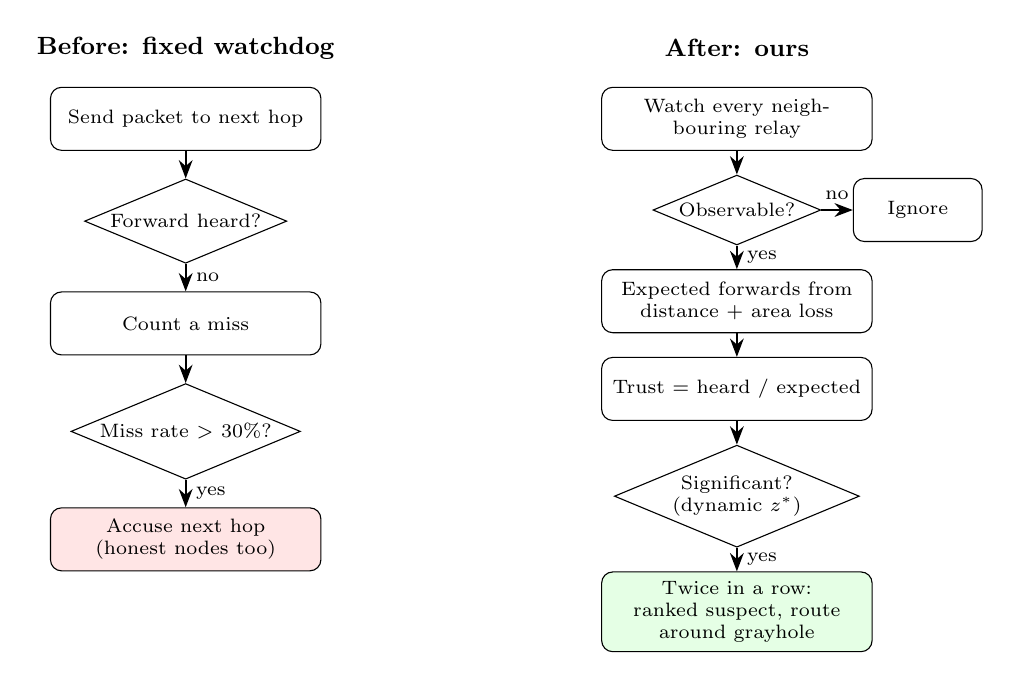
\begin{tikzpicture}[box/.style={draw,rounded corners,align=center,text width=3.2cm,minimum height=0.8cm,font=\scriptsize},dec/.style={draw,diamond,aspect=2.4,align=center,inner sep=1pt,font=\scriptsize},arr/.style={-{Stealth},thick}]
\node[font=\small\bfseries] at (0,0.9) {Before: fixed watchdog};
\node[box] (a1) at (0,0) {Send packet to next hop};
\node[dec,below=0.35cm of a1] (a2) {Forward heard?};
\node[box,below=0.35cm of a2] (a3) {Count a miss};
\node[dec,below=0.35cm of a3] (a4) {Miss rate $>$ 30\%?};
\node[box,below=0.35cm of a4,fill=red!10] (a5) {Accuse next hop\\(honest nodes too)};
\draw[arr](a1)--(a2);\draw[arr](a2)--node[right,font=\scriptsize]{no}(a3);\draw[arr](a3)--(a4);\draw[arr](a4)--node[right,font=\scriptsize]{yes}(a5);
\node[font=\small\bfseries] at (7,0.9) {After: ours};
\node[box] (b1) at (7,0) {Watch every neighbouring relay};
\node[dec,below=0.3cm of b1] (b2) {Observable?};
\node[box,right=0.4cm of b2,text width=1.4cm] (b2x) {Ignore};
\node[box,below=0.3cm of b2] (b3) {Expected forwards from distance + area loss};
\node[box,below=0.3cm of b3] (b4) {Trust = heard / expected};
\node[dec,below=0.3cm of b4] (b5) {Significant?\\(dynamic $z^*$)};
\node[box,below=0.3cm of b5,fill=green!10] (b6) {Twice in a row: ranked suspect, route around grayhole};
\draw[arr](b1)--(b2);\draw[arr](b2)--node[above,font=\scriptsize]{no}(b2x);\draw[arr](b2)--node[right,font=\scriptsize]{yes}(b3);\draw[arr](b3)--(b4);\draw[arr](b4)--(b5);\draw[arr](b5)--node[right,font=\scriptsize]{yes}(b6);
\end{tikzpicture}
\caption{Before and after: the baseline watchdog's decision path and ours.}\label{fig:beforeafter}
\end{figure}

\subsection{System and attacker model}
The standard topology contains 20 static sensors and one sink. Positions and a distance-loss curve are assumed known. All monitors report their counters truthfully, including nodes that maliciously drop relayed packets. An attacker drops each received relayed packet independently with probability $p$; its own source traffic is not attacked. Several attackers mean independently dropping nodes, not coordinated collusion. Ground-truth attacker identities are used only for experiment construction and scoring.

\begin{figure}[H]\centering\setstretch{1}
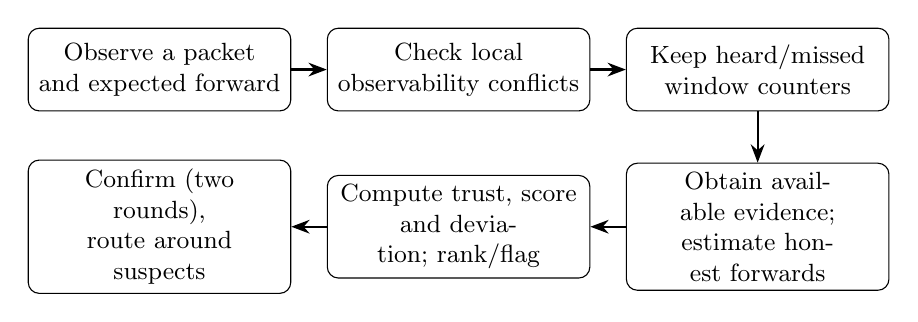
\begin{tikzpicture}[box/.style={draw,rounded corners,align=center,text width=3.1cm,minimum height=1.05cm,font=\small},arr/.style={-{Stealth},thick}]
\node[box] (a) {Observe a packet\\and expected forward};
\node[box,right=0.45cm of a] (b) {Check local\\observability conflicts};
\node[box,right=0.45cm of b] (c) {Keep heard/missed\\window counters};
\node[box,below=0.65cm of c] (d) {Obtain available evidence;\\estimate honest forwards};
\node[box,left=0.45cm of d] (e) {Compute trust, score\\and deviation; rank/flag};
\node[box,left=0.45cm of e] (f) {Confirm (two rounds),\\route around suspects};
\draw[arr](a)--(b);\draw[arr](b)--(c);\draw[arr](c)--(d);\draw[arr](d)--(e);\draw[arr](e)--(f);
\end{tikzpicture}
\caption{Implemented flow. In the live network the sink sees only reports that actually arrive over the acoustic channel, plus its own observations. An excluded window contributes neither a heard nor a missed count.}\label{fig:framework}
\end{figure}

\subsection{Observability checks}
For monitor $M$, sender $A$ and relay $B$, known distances and sound speed estimate the packet's arrival interval at $B$ and the interval in which $M$ expects a forward. The forwarding allowance is 2~s; on the tuning networks 99\% of forwards left within 50~ms and the longest took 1.12~s. It is a configured observation allowance, not a guaranteed queueing bound.

The main rule retains a window only when (C1) the monitor did not transmit during its watch interval, (C3) the monitor did not observe the relay transmitting during the incoming packet's arrival, and (C4) no transmission known to the monitor would overlap that arrival at the relay. These conditions apply to heard forwards and misses alike. Hidden interference and decoding losses remain possible.

A corrupted-frame notification at the monitor (C2) is not an exclusion in the main method. The relay's own attempted forward can cause that notification, while deliberate dropping produces no frame. Excluding it can preferentially remove honest forwarding attempts. Applying C1+C3+C4 is not a proof of unbiased sampling; the remaining selection dependencies require empirical checks.

\subsection{Expected forwards and score}
Let the channel loss at distance $d$ be $e(d)=0.15(d/1500)^2$ within range. For retained window $w$, the channel-only probability of hearing an honest forward is approximated by
\begin{equation}g_w=(1-e(d_{AB}))(1-e(d_{BM})).\end{equation}
For each monitor--relay link $i$, let $n_i$ be retained windows, $O_i$ heard forwards and $G_i=\sum_w g_w$. Its residual loss is
\begin{equation}\kappa_i=\max(0,1-O_i/G_i).\end{equation}
Links with at least five windows and positive $G_i$ enter the estimator. Near, medium and far groups are distance tertiles. For a judged relay $B$, each group's residual loss is the median over other relays' links. If no alternative exists, the group-wide fallback includes its own links. This fallback loses leave-self-out protection.
\begin{equation}
E_i=G_i(1-\kappa_{\mathrm{area},-B}),\qquad
T_B=\frac{\sum_i O_i}{\sum_i E_i},\qquad
S_B=100\max(0,1-T_B).
\end{equation}
If the honest expectation were correct and an independent drop process retained fraction $1-p$, the expected observed count would be $(1-p)E$. This motivates $1-O/E$ as a drop estimate. In practice $E$ is estimated, so the formula is model-based rather than a universal unbiased estimator. Zero expected forwards make a relay unjudgeable. Trust may exceed one; the suspiciousness score is then zero.

\subsection{Dynamic threshold and confirmation}
The raw deviation uses
\begin{equation}
z_B=\frac{\sum_i E_i-\sum_i O_i}{\sqrt{\sum_i E_i\max(0.01,1-E_i/n_i)}}.
\end{equation}
A scale factor $\phi=\max(1,\operatorname{median}(z_B^2)/0.455)$ is computed over judged relays with negative raw $z$. With fewer than two such relays, all judged relays are used. Each deviation is divided by $\sqrt\phi$. For $k$ judged relays, the numerical threshold is $z^*=\Phi^{-1}(1-\alpha/k)$. The relay is flagged only with at least 20 windows, $S_B\geq10$, and corrected $z_B>z^*$.

The expectation, dispersion and number of judged relays can change with the observations. Alpha, the minimum count and the score floor are fixed within an experiment. Correlation between monitors means neither the nominal normal approximation nor its Bonferroni-shaped boundary guarantees a false-alarm probability. We therefore choose alpha on separate tuning networks (topologies 101--106), never on the test networks.

\textbf{Several grayholes: baseline cleaning.} With two or three busy grayholes in one area, the area's normal loss rises, honest relays look better than expected, $\phi$ grows to 50--300 and hides every grayhole, although the grayholes still rank first. The detector therefore removes relays with $S_B\geq10$, and relays already confirmed as suspects, from the area medians and repeats the estimate (at most three times, until stable). On the calibration networks on the tuning networks this raised three-grayhole detection from 4/18 to 13/18 and two-grayhole detection from 9/12 to 12/12.

\textbf{Confirmation.} A relay becomes a suspect only when it is flagged in two consecutive 30-minute rounds, so a single noisy round accuses nobody; a confirmed suspect stays one until the administrator reviews it. The same rule is applied to every compared method.

\subsection{Readable algorithm and implementation}
\begin{quote}\small
\textbf{At a monitor:} open a watch when a packet is sent or overheard toward a relay; record whether its forward is heard; close the watch; assign the outcome and conflicts to a counter bin.\par
\textbf{At a decision:} select eligible counters; calculate channel expectation and area residual losses; calculate each relay's expected forwards and score; correct deviations for empirical dispersion; rank by score and apply the three alarm conditions.\par
\textbf{During response:} every 30 minutes each monitor sends one bundled report; the sink keeps the latest delivered report of every link, runs the detector, confirms suspects over two rounds, gives the administrator the ranked list and routes traffic around the suspects wherever another path exists.
\end{quote}
\texttt{MonitorNode.groovy} handles observations and reports; \texttt{Detectors.groovy} handles scoring; \texttt{Topology.groovy} handles routes. One pipeline (\texttt{run.sh}) calls these shared classes: \texttt{record.groovy} records evidence, \texttt{compare.groovy} replays the sink's decisions for every method on the same evidence, \texttt{network.groovy} runs the live network, and \texttt{plots.py} draws the graphs. The 32 counter bins preserve outcome, sender/overhear status and conflict bits so component variants can reuse identical evidence.

A report is one data frame: a 12-byte header (packet header and busy fraction) and one 17-byte entry per watched relay (identifier, two 32-bit counters, 64-bit expected-forward sum), at most six entries in the 128-byte frame. Reports are jittered over ten minutes after each 30-minute checkpoint and traverse the same lossy network as data. The controller does not read remote agent memory. Route distribution itself remains instantaneous and uncharged.

\section{Experimental Method}\label{sec:experiments}
All experiments run in one pipeline (\texttt{run.sh}). \texttt{record.groovy} simulates the networks and stores every monitor's counters; \texttt{compare.groovy} replays the sink's 30-minute decisions for every method on exactly the same counters; \texttt{network.groovy} runs the live network, in which reports travel over the acoustic channel, the sink detects and confirms suspects and routes traffic around them; \texttt{plots.py} draws the graphs. The fixed watchdog and the CAD-style detector use the same reporting, confirmation and response as ours, so only the detection logic differs.

\begin{table}[H]\centering\small\setstretch{1}
\begin{tabular}{p{4.6cm}p{9.2cm}}\toprule Parameter & Value\\\midrule
Simulator & UnetStack 7.0.0, protocol channel model with distance-dependent loss, Java 8\\
Network & 20 sensors and one sink in 4 km $\times$ 4 km; range 1500 m; sound speed 1500 m/s; 40-sensor and sparse variants\\
Traffic & 0.001--0.01 packets/s per sensor (detection); 0.005 and 0.01 (live network)\\
Grayholes & The 1, 2 or 3 busiest relays, each dropping 30\% of relayed packets (drop-rate sweep 10--100\%)\\
Networks & Tuning: topologies 101--106 (thresholds only); test: topologies 201--210\\
Duration & 6 h recorded runs; 12 h live-network runs; one decision every 30 min\\
Own rules & Fixed watchdog miss rate $>30\%$; CAD-style $z>2$; ours $\alpha=10^{-4}$\\
Same-budget thresholds & At most 5\% of honest relays accused on the no-attack tuning runs: fixed 0.6, CAD-style $z>2.5$, ours $\alpha=10^{-4}$\\
Response & Confirmed suspects stop relaying wherever another path exists\\\bottomrule
\end{tabular}
\caption{Simulation parameters.}\label{tab:params}
\end{table}

Detection metrics are the fraction of grayholes confirmed by the end of a run and the honest relays confirmed as suspects. Network metrics are the delivery ratio and throughput (honest data packets delivered per hour) including all report traffic. A topology is the independent unit; intervals are 95\% $t$-intervals over the ten test topologies, paired by topology where two methods are compared.

\section{Results and Discussion}\label{sec:results}
\subsection{Before and after}
Figure~\ref{fig:fig1} summarises the whole evaluation. Under attack, the fixed watchdog catches every grayhole only by accusing 7.2 honest nodes per run, and routing around them costs most of what it gains: delivery rises only from 45.6\% to 47.0\%. CAD-style accuses fewer honest nodes (0.8) but misses 42\% of the grayholes. Ours catches 95\% of the grayholes while accusing 0.3 honest nodes per run, and gives the highest delivery ratio (49.7\%) and throughput (200.5 against 186.8 packets per hour without defence).
\begin{figure}[H]\centering
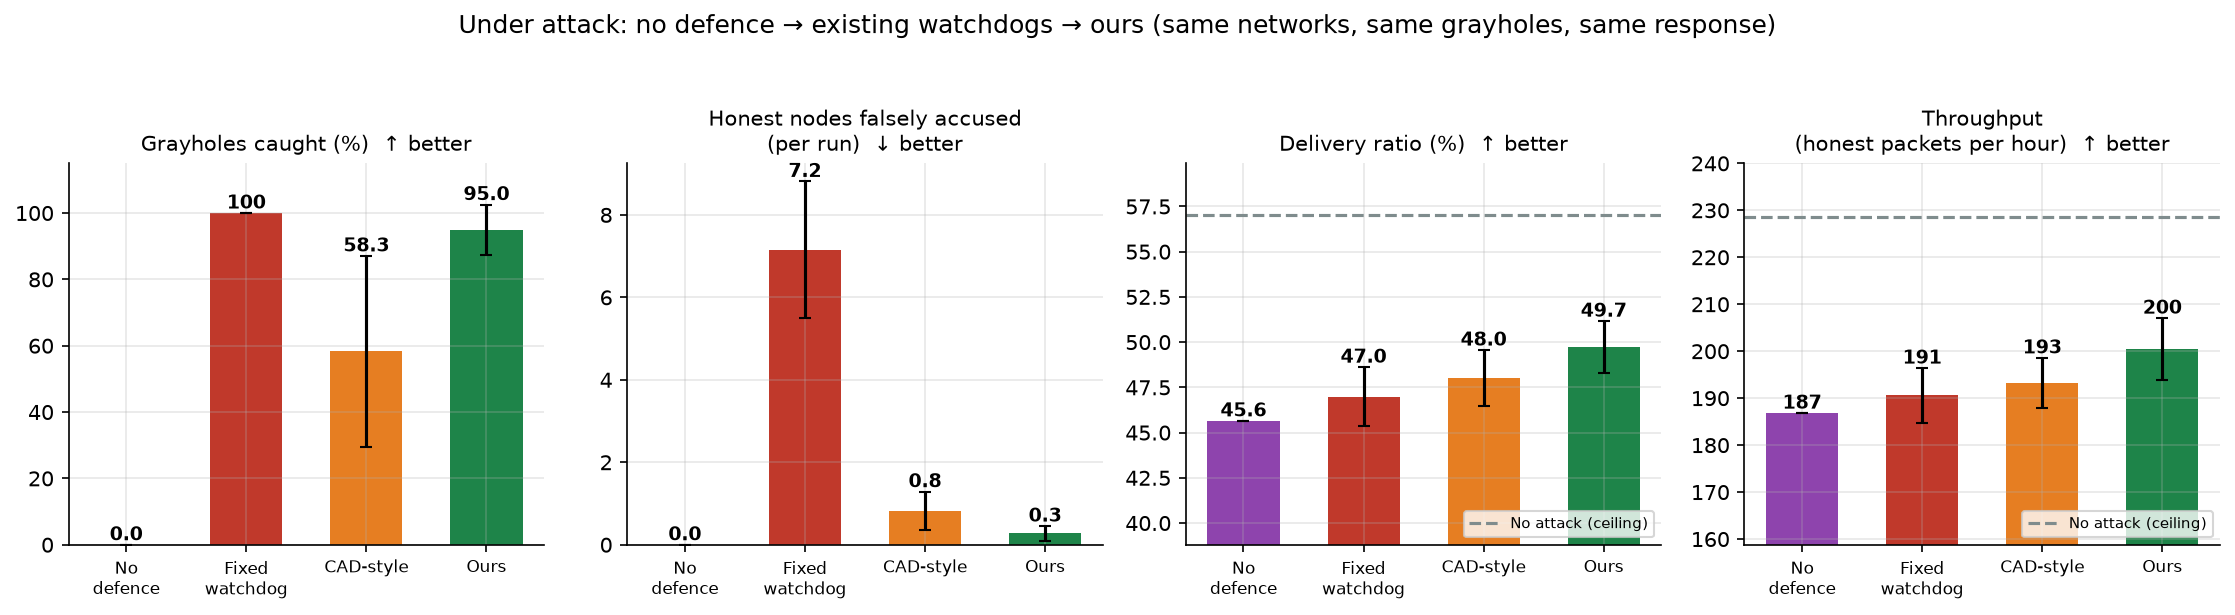
\includegraphics[width=\textwidth]{figs/fig1_before_after.png}
\caption{Before and after in the live network: grayholes caught, honest nodes accused, delivery ratio and throughput (12 h, ten test topologies, 1 grayhole at two loads and 2 and 3 grayholes pooled). The dashed line is the same networks without attack.}\label{fig:fig1}
\end{figure}

\subsection{Why the fixed watchdog accuses honest nodes}
Figure~\ref{fig:fig2} shows honest relays confirmed as suspects as traffic grows. With no attacker at all, the fixed watchdog accuses 1.0 honest relay per run at the lowest load and 6.2 at the highest, because collisions and half-duplex deafness grow with traffic and are counted as drops. CAD-style accuses 0.3--0.7. Ours accuses 0--0.1, because unobservable windows are ignored and each link is compared with the loss it is expected to show.
\begin{figure}[H]\centering
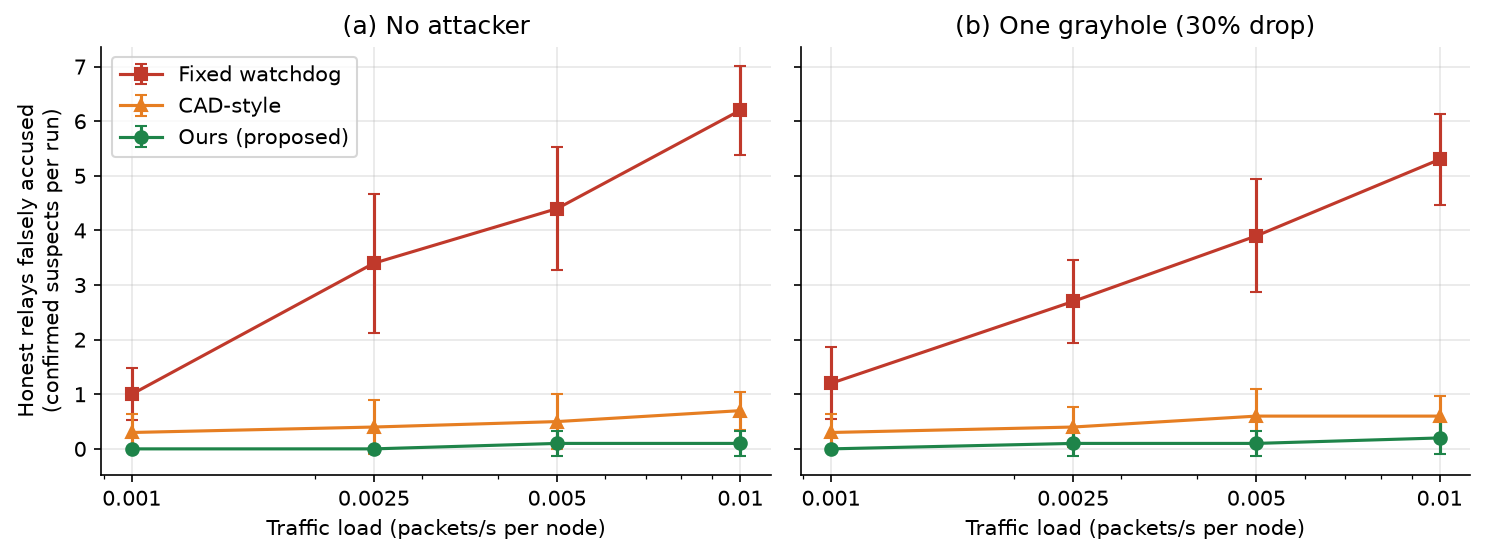
\includegraphics[width=\textwidth]{figs/fig2_false_accusations.png}
\caption{Honest relays falsely accused per run against traffic load, each method with its own rule (6 h, ten test topologies).}\label{fig:fig2}
\end{figure}

\subsection{Grayhole detection in every scenario}
Figure~\ref{fig:fig3}(a) is the fair contest: every method's threshold is tuned on the separate tuning networks so that at most 5\% of honest relays are accused without an attacker. Ours detects 90\% of single grayholes over four loads (CAD-style 58\%, fixed 22\%), 90\% with traffic hotspots, 100\% in the 40-node network, 95\% with two grayholes (65\%, 40\%) and 77\% with three (77\%, 40\%). Figure~\ref{fig:fig3}(b) shows the same methods with their own rules: the fixed watchdog reaches 100\% detection only by accusing 41--71\% of honest relays. Ours accuses no honest relay in the two- and three-grayhole cases. In the hotspot and 40-node networks ours accuses about 10\% of honest relays, more than the fixed watchdog at the same budget.
\begin{figure}[H]\centering
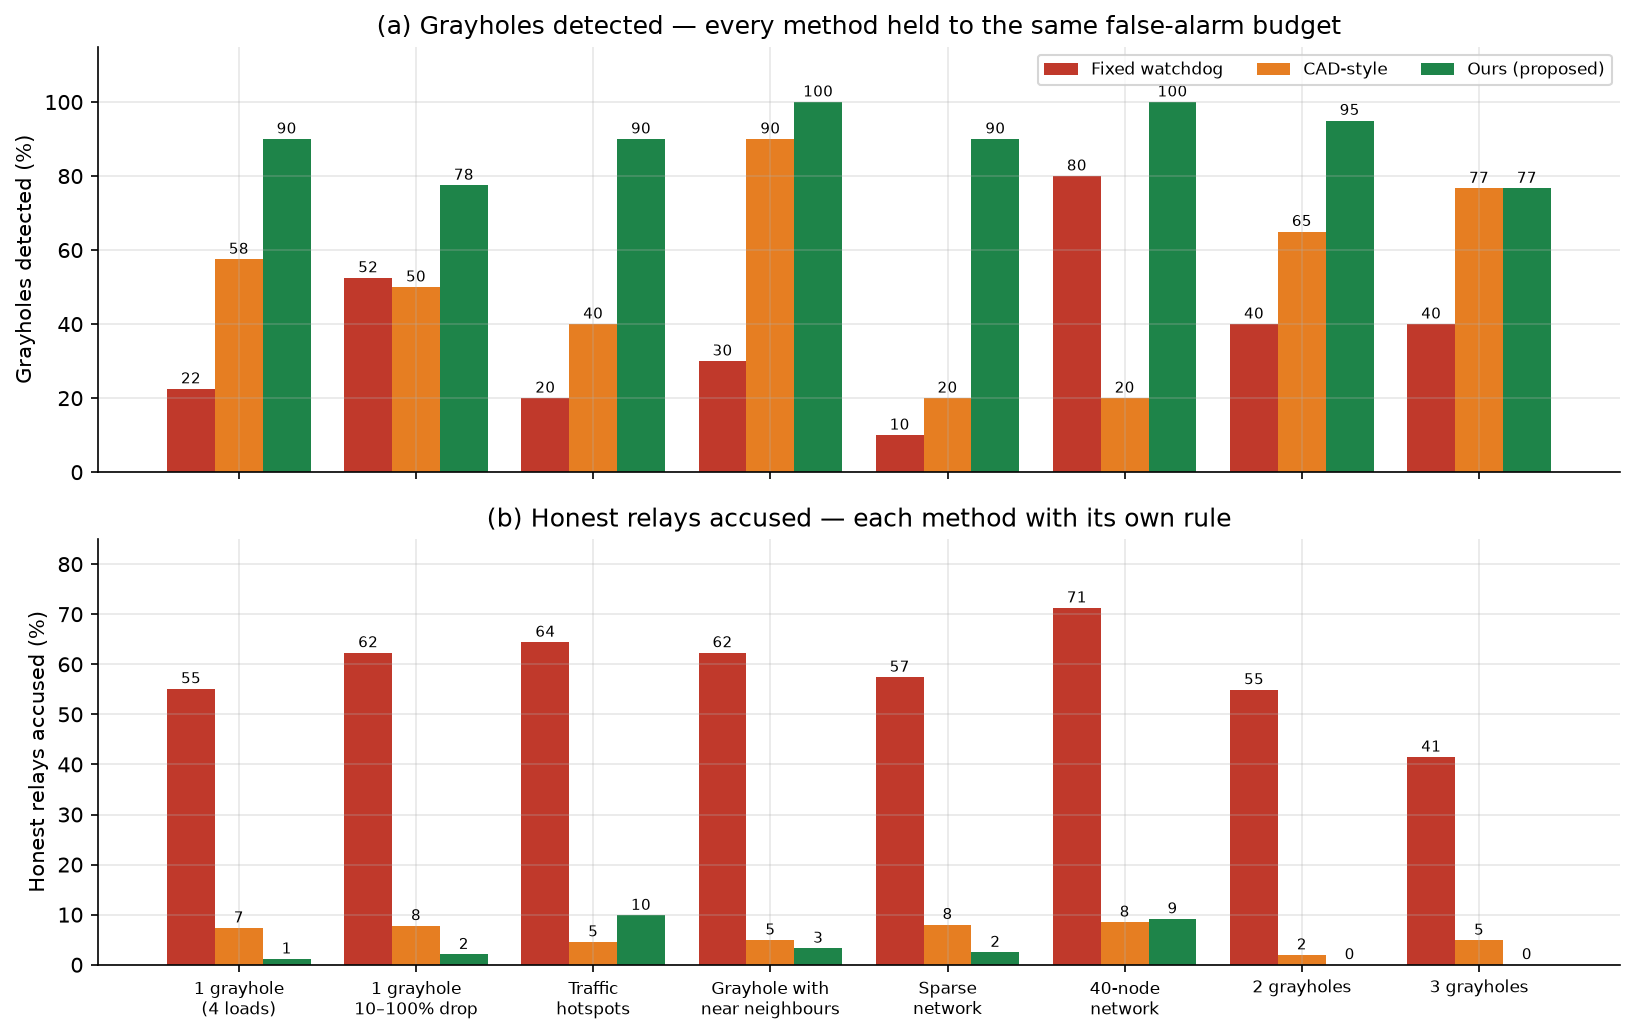
\includegraphics[width=\textwidth]{figs/fig3_detection.png}
\caption{(a) Grayholes detected with all methods held to the same false-alarm budget; (b) honest relays accused with each method's own rule.}\label{fig:fig3}
\end{figure}

\subsection{Ranked suspect list}
Figure~\ref{fig:fig4}(a) is the list the administrator receives for a network with three grayholes. The three grayholes rank first with estimated drop rates of 38.9\%, 32.1\% and 28.2\% and are confirmed as suspects; every honest relay is estimated at 0--0.2\%. Figure~\ref{fig:fig4}(b) shows that the estimate follows the true drop rate (7.2, 18.5 and 47.3\% for 10, 20 and 50\%), while CAD-style underestimates moderate dropping.
\begin{figure}[H]\centering
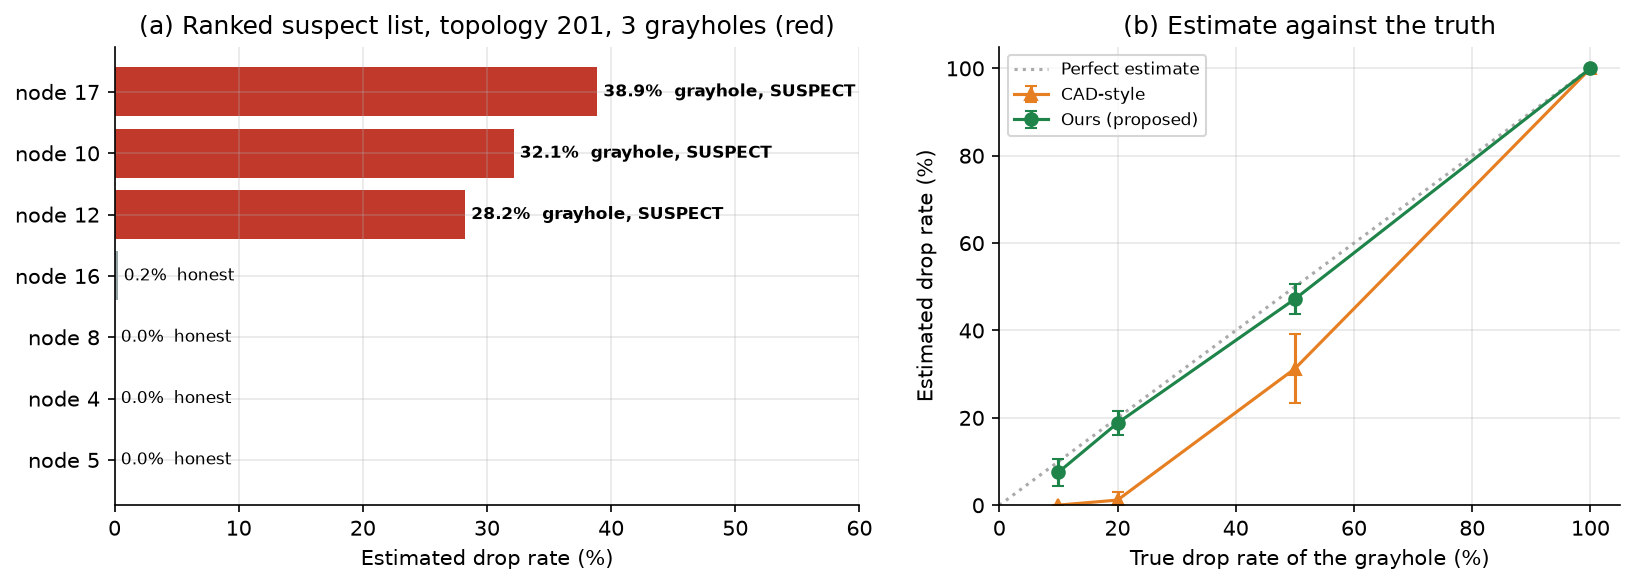
\includegraphics[width=\textwidth]{figs/fig4_suspect_list.png}
\caption{(a) Ranked suspect list for one test network with three grayholes; (b) estimated against true drop rate.}\label{fig:fig4}
\end{figure}

\subsection{Network performance}
Figure~\ref{fig:fig5}(a) breaks the live-network delivery down by setting. Ours has the highest delivery in all four. Compared with no defence on the same topologies it gains 4.0, 1.7, 5.6 and 4.9 percentage points (significant except at the higher load), and compared with the fixed watchdog 4.0 points with two and with three grayholes. Against CAD-style ours is ahead in every setting, but by 0.7--2.7 points, within the uncertainty. Figure~\ref{fig:fig5}(b) shows the mechanism over time with three grayholes: delivery falls when the attack starts and climbs back once ours has confirmed the grayholes. Figure~\ref{fig:fig5}(c) repeats the experiment with suspects blacklisted instead of avoided: every honest node the fixed watchdog accuses is then lost with the nodes behind it, and its delivery collapses to 23.2\% against 45.6\% without defence. Blacklisting also hurts a correct detector when a grayhole is the only path for many nodes, which is why routing around suspects is the response used here.
\begin{figure}[H]\centering
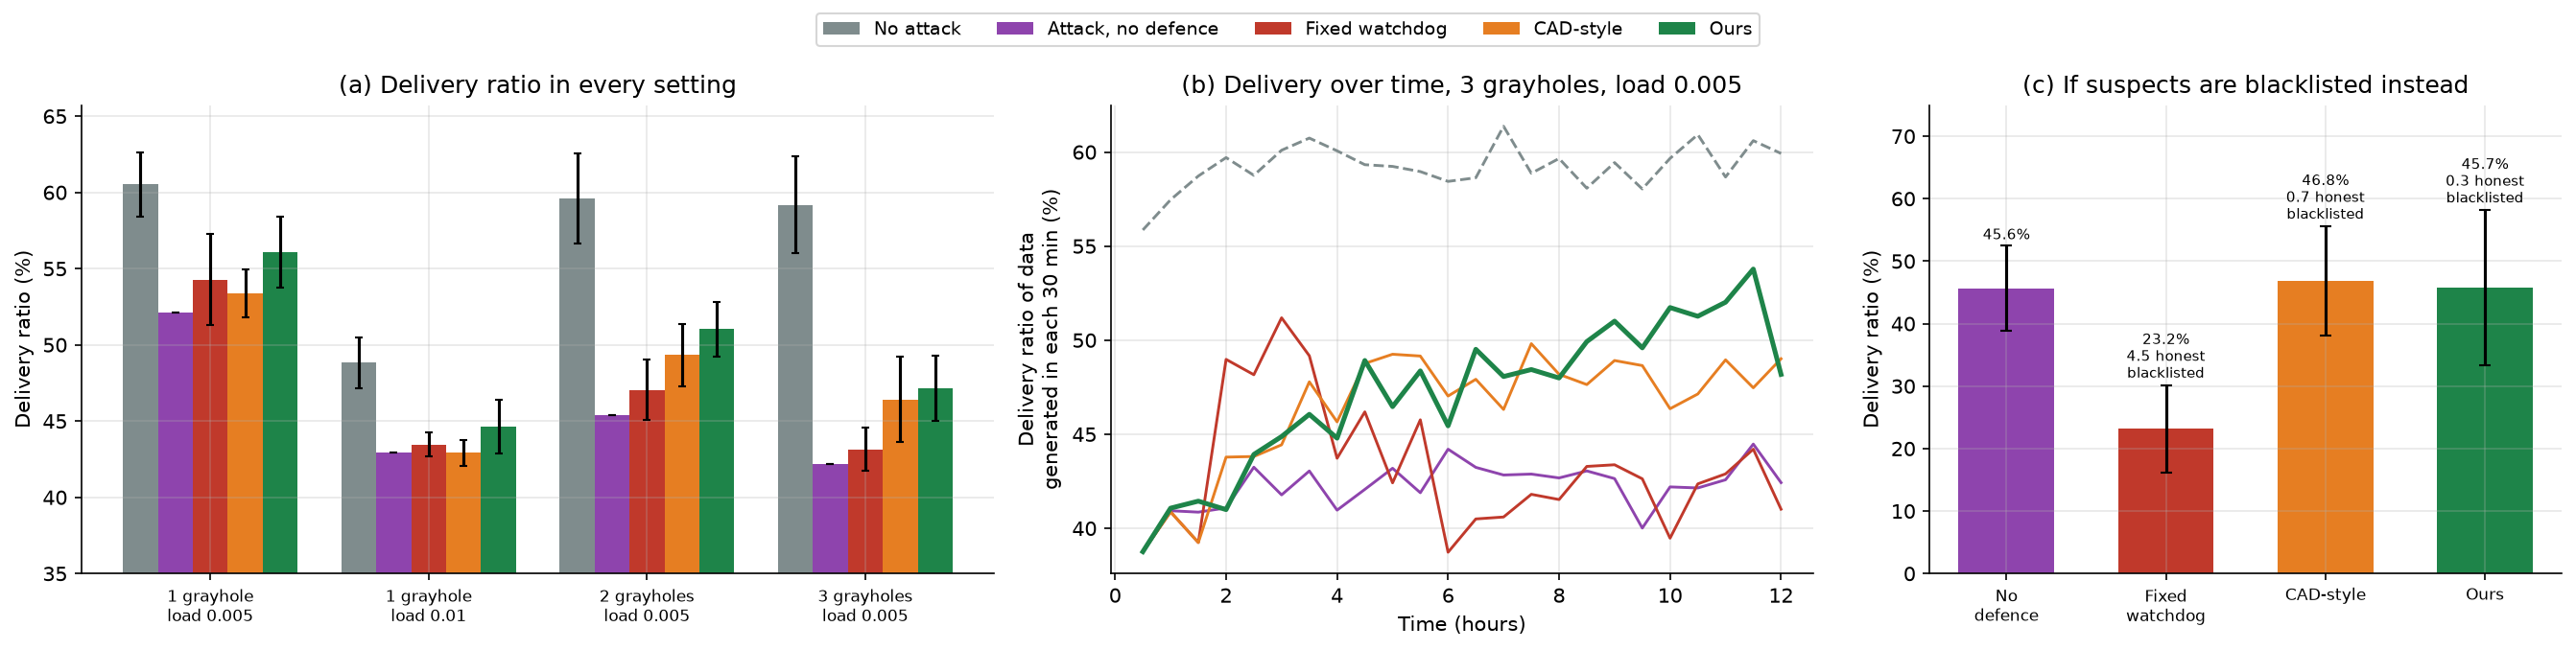
\includegraphics[width=\textwidth]{figs/fig5_network_performance.png}
\caption{Live network: (a) delivery ratio per setting, error bars are paired 95\% intervals against no defence; (b) delivery over time with three grayholes; (c) delivery when suspects are blacklisted.}\label{fig:fig5}
\end{figure}

\subsection{Contribution of each part}
Removing one part at a time, at the same 5\% budget: without baseline cleaning, three-grayhole detection falls from 23/30 to 17/30; using an area average instead of the median gives similar detection (23/30); without the observability filter, detection is similar (37/40 single, 22/30 three grayholes) but honest accusations rise slightly (1.5\% against 1.1\% in the load sweep). With two-round confirmation in place, the filter's contribution is therefore small in these networks; its main effect is visible in the false accusations of Figure~\ref{fig:fig2}, where the methods without it count unobservable windows as drops.

\section{Limitations and Reproducibility}\label{sec:limits}
\begin{enumerate}
\item Static connected topologies, known positions, a known distance--loss curve and truthful monitors; mobility, location error and falsified reports are not evaluated.
\item The CAD-style comparator is an adaptation, and the fixed watchdog follows the published rule, not every detail of its implementation.
\item Ten test topologies per setting; several comparisons are exploratory. Delivery gains over CAD-style are within the uncertainty.
\item Route updates are instantaneous and free in the simulation; report traffic, delay and loss are simulated and counted.
\end{enumerate}
\texttt{./run.sh} regenerates every number and graph from the recorded counters in about an hour; \texttt{./run.sh demo} runs one network with three grayholes in about three minutes and prints the ranked suspect list; \texttt{./run.sh record} also re-records the counters.

\section{Conclusion and Future Work}\label{sec:conclusion}
We implemented an observability-aware, trust-based grayhole detector for underwater acoustic networks in UnetStack and compared it with a fixed watchdog and a CAD-style detector in one pipeline. Judging only observable windows against each link's expected loss, with a dynamic threshold and two-round confirmation, the detector caught 95\% of grayholes while accusing 0.3 honest nodes per run, against 7.2 for the fixed watchdog, and gave the highest delivery ratio and throughput in every live-network setting. The administrator receives a ranked list in which the grayholes come first. Future work should test dishonest monitors, mobility and location errors, larger and denser networks, where ours still accuses about 10\% of honest relays, and a faithful implementation of the published comparators.

\section*{Author review note}
This draft uses AI-assisted code review and manuscript preparation. The team must verify its contents, understand the implementation, and apply the disclosure and authorship rules of the actual submission venue. The supplied article layout is a formatting reference, not confirmation of journal acceptance or venue compliance.

\begin{thebibliography}{9}\small
\bibitem{marti} S. Marti, T. J. Giuli, K. Lai and M. Baker, ``Mitigating routing misbehavior in mobile ad hoc networks,'' in \emph{Proc. ACM MobiCom}, pp. 255--265, 2000. doi: \href{https://doi.org/10.1145/345910.345955}{10.1145/345910.345955}.
\bibitem{cad} D. M. Shila, Y. Cheng and T. Anjali, ``Mitigating selective forwarding attacks with a channel-aware approach in WMNs,'' \emph{IEEE Transactions on Wireless Communications}, vol. 9, no. 5, pp. 1661--1675, 2010. doi: \href{https://doi.org/10.1109/TWC.2010.05.090700}{10.1109/TWC.2010.05.090700}.
\bibitem{brc} B. R. Chandavarkar and N. Suresh, ``Demonstration of selective forwarding attack and detection mechanism in UnetStack3,'' in \emph{Proc. ICCCNT}, pp. 1--6, 2021. doi: \href{https://doi.org/10.1109/ICCCNT51525.2021.9580125}{10.1109/ICCCNT51525.2021.9580125}.
\bibitem{han} D. Han, X. Du, L. Wang, X. Liu and X. Tian, ``Trust-aware and fuzzy logic-based reliable layering routing protocol for underwater acoustic networks,'' \emph{Sensors}, vol. 23, no. 23, art. 9323, 2023. doi: \href{https://doi.org/10.3390/s23239323}{10.3390/s23239323}.
\bibitem{unet} UnetStack, \emph{UnetStack Handbook}, ``Physical,'' \url{https://unetstack.net/handbook/305_phy.html}, accessed 12 October 2026.
\end{thebibliography}
\end{document}
